\documentclass[tikz,border=10pt]{standalone}
\usepackage{tikz}
\usetikzlibrary{arrows.meta,positioning}

\tikzset{
  stepbox/.style={draw=blue!70!black, line width=1.2pt, rectangle, rounded corners=2pt, minimum width=2.8cm, minimum height=1.1cm, align=center, fill=none},
  signal/.style={->, line width=1.2pt, draw=black!80, >=Stealth}
}

\begin{document}
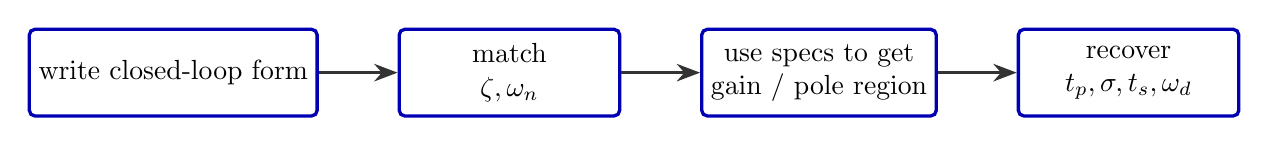
\begin{tikzpicture}[node distance=1.0cm]
  \node[stepbox] (a) {write closed-loop form};
  \node[stepbox, right=of a] (b) {match\\$\zeta,\omega_n$};
  \node[stepbox, right=of b] (c) {use specs to get\\gain / pole region};
  \node[stepbox, right=of c] (d) {recover\\$t_p,\sigma,t_s,\omega_d$};
  \draw[signal] (a) -- (b);
  \draw[signal] (b) -- (c);
  \draw[signal] (c) -- (d);
\end{tikzpicture}
\end{document}
